\section{Preliminaries}
For $m,n,r\in\bbN$ we write $m =_r n$ iff $m=n$ or $m,n>r$.

\subsection{Logic on Graphs and Words}
Let $A$ be a finite set of labels. An \emph{edge-labeled graph} is a tuple $G=(V^G,(E_a^G)_{a\in A})$ where $V$ is the set of vertices and $E_a^G \subseteq V\times V$ is the set of $a$-labeled edges. 
A \emph{word-structure} over $A$ is a tuple $W = (\{0,\ldots, n-1\}, \leq^W, (P_a^W)_{a\in A})$ where $\leq^W$ is the usual order on $\{0,\ldots,n-1\}$, and $(P_a^W)_{a\in A}$ is a partition of $\{0,\ldots, n-1\}$ (some of the sets $P_a^W$ may be empty). Whenever we use logic to describe properties of a word $w$ then the formula is evaluated on the corresponding word structure $W$. 

Let $\tau = \{R_1,\ldots,R_m, c_1, \ldots, c_n\}$ where $R_i$ is a relation symbol of arity $r_i$ and $c_j$ is a constant symbol.
\emph{First-order formulas} (over the vocabulary $\tau$) are build up
from variables and constant symbols $\{x_i \mid i\in \bbN \}\cup \{c_1,\ldots,c_n\}$, the edge relation symbols $\{R_1,\ldots, R_m\}$, the equality symbol $=$, the Boolean connectives
$\{\lnot,\vee,\wedge, \to \}$,
quantifiers $\{\forall, \exists \}$, and the bracket symbols
$\{(,) \}$. 
We write $G\models \phi$ to denote that the formula $\phi$ is satisfied by the structure $G$.
The \emph{quantifier rank} $\qr(\phi)$ of a formula $\phi$
is the maximal nesting depth of quantifiers within $\phi$. Two structures
$G$ and $H$ are \emph{$r$-equivalent} (denoted $G\equiv_r H$) if they
cannot be distinguished by any formula of quantifier rank $\le r$. 
For a structure $G$ and two tuples $\vec{p}, \vec{q} \in (V^G)^m$ we write $\vec{p} \equiv_r^G \vec{q}$ or say that $\vec{p}$ and $\vec{q}$ are $r$-equivalent in $G$
whenever $G\models \phi(\vec{p}) \Leftrightarrow G\models\phi(\vec{q})$ for all first-order formulas $\phi$ with $m$ free variables and
quantifier rank at most $r$. For all the above notations we adopt the convention that we omit superscripts whenever this should not lead to any confusion. For instance we write 
$\vec{p} \equiv_r \vec{q}$ when the underlying structure $G$ is clear from the context. 

The $r$-type of a structure $G$ is the set of all first-order sentences $\phi$ of quantifier rank at most $r$ such that $G\models \phi$. It is well known that there are up to equivalence only
finitely many sentences of quantifier rank at most $r$. Hence the $r$-type of a formula can be characterized by a sentence, which has also quantifier rank $r$. 

\emph{Ehrenfeucht-Fra\"\i{}ss\'e-relations} for a graph $G = (V, (E_a)_{a\in A})$ are a system $(\calE^r_m)_{r,m\in\bbN}$ where  $\calE^r_m$ is an equivalence relation on $V^m$ and
the following is true for all $r,m\in\bbN$ and $\vec{p},\vec{q} \in V^m$:
\begin{itemize}
	\item If $(p_1,\ldots,p_m) \calE^0_m (q_1,\ldots,q_m)$ then the mapping $p_i \mapsto q_i$ is a partial isomorphism, that is $p_i= p_j \Leftrightarrow q_i=q_j$ and
	$(p_i,p_j)\in E_a \Leftrightarrow (q_i,q_j) \in E_a$ for all $1\leq i,j\leq m$ and all $a\in A$.
	\item If $\vec{p} \calE^{r+1}_m \vec{q}$ then for every $p\in V$ there exists a $q\in V$ such that $(\vec{p}, p) \calE^r_{m+1} (\vec{q}, q)$.
\end{itemize}

Ehrenfeucht-Fra\"\i{}ss\'e-relations are useful to identify $r$-equivalent tuples in a graph. This is formalized in the following theorem.
\begin{theorem}[\!\!\cite{Fra54,Ehr61}]
	Let $G$ be a graph, $(\calE^r_m)_{r,m\in\bbN}$ Ehrenfeucht-Fra\"\i{}ss\'e-relations for $G$, and $\vec{p}, \vec{q}$ $m$-tuples of nodes from $G$. If $\vec{p} \calE^r_m \vec{q}$ then 
	$\vec{p} \equiv_r \vec{q}$.
\end{theorem} 

\subsection{Combinatorics on Words}
Let $A$ be an alphabet. We use $\preceq$ to denote the \emph{prefix-relation} and $\sqsubseteq$ for the \emph{suffix-relation} on $A^\ast$.  If $u= vw$ we write $v^{-1}u = w$ and
$uw^{-1} = v$.
Let $\pref_r(u)$ denote the maximal prefix of $u$ of length at most $r$. For $u,v\in A^\ast$ let $u \sqcap v$ denote the largest suffix of $u$ that is also a prefix of $v$.

In a first lemma we prove that the complementary prefix and suffix of $u$ resp.~$v$ wrt.~$u\sqcap v$ can be shortened to words of length at most $2r$ having the same prefixes and suffixes:

\begin{lemma}\label{lem:short_ends_construction}
	Let $r\in\bbN$ and $u,v,w \in A^\ast$ with $uw\sqcap wv = w$. %such that the period of $w$ has length at least $2$. 
	Then there are words $u',v'$ of length $\leq 2r$ such that 
	
	\begin{minipage}{0.45\linewidth}
	\begin{itemize}
		\item $\suf_r(uw) = \suf_r(u'w)$,
		\item $\suf_r(wv) = \suf_r(wv')$,
	\end{itemize}
    \end{minipage}
    \begin{minipage}{0.45\linewidth}
    	\begin{itemize}
    		\item $\pref_r(wv) = \pref_r(wv')$,
    		\item $u'w\sqcap wv' = w$.
    	\end{itemize}
    \end{minipage}
\end{lemma}
\begin{proof}
	Set $u'=\suf_r(u)$. Additionally, if $|v|\leq 2r$ set $v':=v$, and otherwise, set $v':=\pref_r(v)\suf_r(v)$. Then the first three equations are obviously satisfied. Now assume $u'w\sqcap wv'\neq w$, i.e., there is $w'\in A^*$ with $|w'|>|w|$, $w'\preceq wv'$, and $w'\sqsubseteq u'w$. Since $|u'w|\leq r+|w|$ we have $w'\preceq w\pref_r(v)\preceq wv$. Additionally, we have $w'\sqsubseteq u'w\sqsubseteq uw$ implying $|uw\sqcap wv|\geq|w'|>|w|$. This is a contradiction to the definition of~$w$.
\end{proof}

A \emph{period} of a word $u$ is a word $v$ such that $u \preceq v^\omega$. Obviously every word $u$ has a unique smallest period, which we denote by $\root{u}$. The \emph{left-exponent} of $u$ in $v$ is the largest number $n$ such that $v= u^nw$, and it is denoted by $\lexp(u,v)$. The \emph{right-remainder}, $v\mod u$,  of $v$ with respect to $u$ is defined as $(u^{\lexp(u,v)})^{-1}v$, that is the unique $w$ such that $v= u^{\lexp(u,v)}w$.  In particular we have $v= \root{v}^{\lexp(\root{v}, v)}(v \mod \root{v})$ for every $v\in A^\ast$. A word $u$ is \emph{primitive} if there is no $v$ with
$|v| < |u|$ and $u = v^n$ for some $n\in\bbN$.
For $u,v\in A^\ast$ let $u\Delta v = (y,z)$, where $y,z$ are minimal such that there exists an $x$ with $u=xy$ and $v=xz$. For $\vec{v}, \vec{w}\in(A^\ast)^k$ let 
$\vec{v}\Delta\vec{w} = (v_1\Delta w_1,\ldots, v_k\Delta w_k) \in (A^\ast)^{2k}$ and $|\vec{w}| \coloneq \sum_{i=1}^{k}|w_i|$. 

\begin{definition}
	Let $u\in A^\ast$ be a word. A word $v\in A^*$ is a \emph{border} of $u$ (denoted by $v\presuf u$) if $v \precneq u$ and $v \sqsubsetneq u$. A \emph{border-decomposition} of $u$ is a sequence of words $\epsilon = u_0,u_1,\ldots, u_n = u$ such that for all $0\leq i < n$ it holds that
	$u_i \presuf u_{i+1}$. A border-decomposition $u_0,u_1,\ldots, u_n $ is \emph{complete} if there is no $1\leq i< n$ and $v\in A^\ast$ with $u_i \presuf v \presuf u_{i+1}$.
\end{definition}

Hence, a complete border-decomposition of $u\in A^*$ is the sequence of all borders of $u$ ordered by word length. So, it is easy to observe that each word $u\in A^*$ has exactly one complete border-decomposition.

%\begin{observation}
%	Every word $w\in A^\ast$ has a unique complete canon-decomposition.
%\end{observation}
%\begin{proof}
%	Obviously, every word $w$ possesses at least one complete canon-decomposition. Now suppose $\vec{u} = (u_0,\ldots,u_m)$ and $\vec{v}=(v_0,\ldots,v_n)$ are two distinct complete canon-decompositions of
%	a word $w\in A^\ast$. W.l.o.g. assume that $n \leq m$. We claim that there is an $0\leq i \leq n$ with $u_i \neq v_i$. Because otherwise it follows from $w= u_n = v_n$ that    
%	$\vec{u}$ and $\vec{v}$ have the same length $n$ and this, in turn, implies that they are identical since $u_i=v_i$ for all $0\leq i\leq n$. Now choose the smallest $i$ between $0$ and $n$ such that $u_i \neq v_i$. As $u_0 = \epsilon = v_0$ it holds that $i>0$. Hence $u_{i-1}, v_{i-1}$ are defined and $u_{i-1} = v_{i-1}$. Since $u_i, v_i \preceq w$ and $u_i \neq v_i$ it must be the case that $|u_i| \neq |v_i|$. Again w.l.o.g. assume that $|u_i| < |v_i|$. Then  $u_i, v_i \preceq w$, $u_i, v_i \sqsubseteq w$ and $|u_i| < |v_i|$, which implies $u_i \presuf v_i$. Therefore 
%	$v_{i-1} = u_{i-1} \presuf u_i \presuf v_i$ in contradiction to the completeness of $\vec{v}$!
%\end{proof}

\begin{example}
	The  complete border-decomposition of $ababa$ is $(\epsilon, a, aba, ababa)$.
\end{example}

%\begin{definition}
%	A word $u$ is \emph{periodic} if $u=v^n$ for some $v\in\Sigma^+$ and $n>1$. Otherwise $u$ is primitiv. We say that $u$ is almost periodic if $u= (vw)^nv$ for some $n\geq 1$,  $v\in \Sigma^\ast$, and $w\in\Sigma^+$.  We write $\sqrt{u}^{\ast}$ for the unique pair $(v,w) \in \Sigma^\ast\times\Sigma^+$ such that
%   $vw$ is primitive and $u = (vw)^nv$ for some $n\geq 1$.
%
%\end{definition}

%\begin{lemma}
%	Let $\vec{u} = (u_0,\ldots,u_n)$ be a complete border-decomposition. Then $\root{u_{i+1}} = u_{i+1}u_i^{-1}$ for all $0\leq i < n$. 
%\end{lemma}
%\begin{proof}
%	Fix some $0\leq i < n$ and let $v:= u_{i+1}u_i^{-1}$. Let us verify first that $v$ is indeed a period of $u_{i+1}$. If $2|u_i| \leq |u_{i+1}|$ then $u_{i+1} = u_iwu_i$ for some $w\in\Sigma^\ast$. 
%	Hence $v= u_iw$ and $u_{i+1} \preceq (u_iw)^\omega = v^\omega$. Otherwise  $2|u_i| > |u_{i+1}|$ and therefore the $u_i$-prefix and the $u_i$-suffix of $u_{i+1}$ overlap. We can use this overlap to 
%	show via a simple induction that the situation is as depicted in Fig.~\ref{fig:root}.
%	\begin{figure}[h]
%		\centering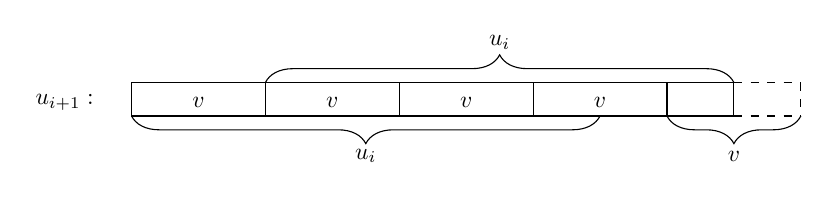
\begin{tikzpicture}[scale=0.85,every node/.style={scale=0.85}]
	\node at (-1, .2) {$u_{i+1}:$};
	\node at (1, .2) {$v$};
	\node at (3, .2) {$v$};
	\node at (5, .2) {$v$};
	\node at (7, .2) {$v$};
	\draw [decorate,decoration={brace,amplitude=10pt}] (10,0) -- (8, 0) node [black,midway,yshift=-.6cm] {$v$};
	\draw (0,0) rectangle (9, .5);
	\draw [decorate,decoration={brace,amplitude=10pt}] (7,0) -- (0, 0) node [black,midway,yshift=-.6cm] {$u_i$};
	\draw [decorate,decoration={brace,amplitude=10pt}] (2,0.5) -- (9, 0.5) node [black,midway,yshift=.6cm] {$u_i$};
	\draw (2,.5) -- (2,0);
	\draw (4,.5) -- (4,0);
	\draw (6,.5) -- (6,0);
	\draw (8,.5) -- (8,0);
	\draw[dashed] (10,.5) -- (10,0);
	\draw[dashed] (9,.5) -- (10,.5);
	\draw[dashed] (9,0) -- (10,0);   
\end{tikzpicture}
%		\caption{\label{fig:root}}
%	\end{figure}
%
%	Now suppose that $|\root{u_{i+1}}| < |v|$. Then let $u_i' \coloneq \root{u_{i+1}}^{\lexp(\root{u_{i+1}}, u_{i+1}) -1}(u_{i+1} \mod \root{u_{i+1}})$.
%	Then $u_i' \presuf u_{i+1}$ and $|u_i'| = |u_{i+1}| - \root{u_{i+1}} > |u_{i+1}| - |v| = |u_i|$. Hence $u_i\presuf u_i' \presuf u_{i+1}$ contradicting the completeness of $\vec{u}$! 
%\end{proof}

From the complete border-decomposition of a word~$w$ we derive the so called skeleton of~$w$ containing the inner words $v$ of all bordered words $uvu$ in $w$.

\begin{definition}
	Let $w\in A^\ast$ and $\vec{w} = (w_0,\ldots,w_n)$ be the complete border-decomposition of $w$. The \emph{$r$-skeleton} of $w$, denoted by $\calS_r(w)$, is the word of length $n$ over the alphabet $\Gamma = A^{\leq r}$ with $\calS_r(w)[i] = \pref_r(w_i^{-1}w)$ for each $0\leq i\leq n-1$. Note that $w_i^{-1}w$ is always defined since $w_i\preceq w$.
	\begin{figure}[H]
	\begin{center}
		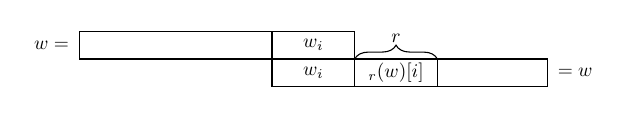
\begin{tikzpicture}[scale=0.7,every node/.style={scale=0.7}]
	\path[draw] (0,0) rectangle (3.5,0.5);
	\path[draw] (3.5,0) rectangle (5,0.5);
	\path[draw] (6.5, 0) rectangle (8.5, -.5);
	\path[draw] (3.5,0) rectangle (5,-0.5);
	\path[draw] (5, 0) rectangle (6.5, -.5);
	\draw[draw, decorate, decoration={brace,amplitude=5pt}] (5, 0) -- node[above, yshift= 5pt] {$r$} (6.5, 0);
	
	
	\node at (4.25, 0.25) {$w_i$};
	\node at (4.25, -0.25) {$w_i$};
	\node at (5.75, -0.25) {$\calS_r(w)[i]$};
	\node at (-.5, .25) {$w=$};
	\node at (9, -.25) {$=w$};
	\end{tikzpicture}
	\end{center}\label{fig:skeletondef}\caption{Definition of $\calS_r(w).$}
    \end{figure}
\end{definition}
Note that it is convenient for our purpose to consider $\calS_r(w)$ to be a word over an alphabet, which in itself consists of words of bounded length rather than to consider $\calS_r(w)$ as a sequence of words.

\begin{example}
	Let $u= bababa$ and $v=ababab$. Then $u\sqcap v = ababa$ and the complete border-decomposition of $u\sqcap v$ is $(\epsilon, a, aba, ababa)$. The $2$-skeleton of $u\sqcap v$ is the word depicted below.

	\begin{center}
		\begin{tikzpicture}[scale=0.85]
			\node[] (0) {$ab$};
			\node[ right=of 0] (1) {$ba$};
			\node[ right=of 1] (2) {$ba$};
			
			\path[ ->,>=latex'] (0) edge (1)
			(1) edge (2);
		\end{tikzpicture}
	\end{center}\label{fig:skeletonex}
\end{example}

Skeletons will play a crucial role in Section \ref{sec:decidability}. 
We will prove the decidability of the Cayley-graph of a queue-monoid by  translating back and forth between 
an Ehrenfeucht-Fra\"{\i}ss\'{e} game played on the Cayley-graph (presented as EF-relations) and games played on certain skeletons which are derived from the game played on the Cayley-graph. 

\begin{restatable}{mylem}{instantiation}\label{lem:short_from_skeleton}
	Let $r\in\bbN$, $w\in A^*$ and $n\in\bbN$ be the length of $\calS_r(w)$. Then a word $v\in A^*$ can be constructed from $w$ such that $|v|=\calO(2^{nr})$ and $\calS_r(w)=\calS_r(v)$.
\end{restatable}
\begin{proof}
	Let $\vec{w}=(w_0,\dots,w_n)$ be the complete border-decomposition of~$w$. At first, assume $|\calS_r(w)[n-1]|<r$ (i.e., the last component is small). Then there are two possibilities: on the one hand $w=w_{n-1}xw_{n-1}$ and $|xw_{n-1}|<r$. In this case we have $|w|<2r=\calO(2^{nr})$. On the other hand we have $w=xw_{n-1}=w_{n-1}y$ where $|x|=|y|<\min\{|w_{n-1}|,r\}$, i.e., the prefix and the suffix $w_{n-1}$ overlap in $w_n$. Then it is easy to see that $x$ is a period of $w_{n-1}$ and of $w_n$. Concretely, there is a prefix $p$ of $x$ and a number $k\in\bbN$ such that $w=x^kp$ and $w_{n-1}=x^{k-1}p$. In particular, all word $x^ip$ with $1\leq i\leq k$ are borders of $w$ which implies $k\leq n$. Hence we have $|w|\leq|x|\cdot(k+1)\leq r\cdot(n+1)=\calO(2^{nr})$. Therefore, in both cases we are ready and we can assume $|\calS_r(w)[n-1]|$ from now on.
	
	We construct~$v$ inductively as follows: We set $v_0:=\epsilon$. Now let $a,b\in A$ be distinct with $\calS_r(w)[0]\in aA^*$. Then $x\presuf\calS_r(w)[0]b^{2n+r}$ implies $x=\epsilon$. Hence, we set, for $0\leq i<n$, $v_{i+1}:=v_ix_iv_i$ where $x_i=\calS_r(w)[i]\,b^{n-i}a^ib^{n+r}$. Finally, we set $v:=v_{n}$.
	
	One can show the following two properties:
	\begin{alphaenumerate}
		\item For each $0\leq i\leq n$ $\root{v_{i+1}}=v_ix_i$ and
		\item $\vec{v}=(v_0,\dots,v_{n})$ is a complete border-decomposition of $v$.
	\end{alphaenumerate}
Finally, let $0\leq i<n$. Then we have
	\[\calS_r(v)[i]=\pref_r(\inv{v_i}v)=\pref_r(\calS_r(w)[i]\,s)=\calS_r(w)[i]\]
	for some $s\in A^*$, i.e., $\calS_r(v)=\calS_r(w)$. Additionally, we have $|v_i|=2|v_{i-1}+2n+2r$ for $1\leq i\leq n$ and $|v_0|=0$ which results in $|v|=|v_n|=(2^n-1)(2n+2r)=\calO(2^{nr})$.
\end{proof}

Let $V\in (A^{\leq r})^*$ be the $r$-skeleton of some word $w\in A^*$. We call the word $v\in A^*$ constructed in the proof of Lemma~\ref{lem:short_from_skeleton} the \emph{$r$-instantiation of $V$}.